\documentclass[a4paper,10pt]{amsart}
\usepackage[utf8]{inputenc}
\usepackage{amssymb}
\usepackage{amsmath}
\usepackage{tikz}
\usepackage{color}

\begin{document}

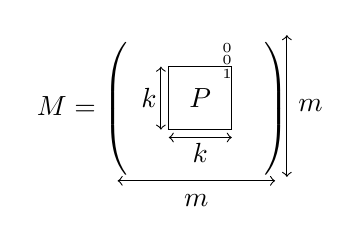
\begin{tikzpicture}
  % Matrix delimiters
  \node at (-0.65,0) {$M = $};
  \node at (0,0) {$\left(\vphantom{\rule{0cm}{1cm}} \right.$};
  \node at (2,0) {$\left.\vphantom{\rule{0cm}{1cm}} \right)$};

  % Submatrix P: draw rectangle and label
  \draw (0.65,-0.3) rectangle (1.45,0.5);
  \node at (1.05,0.1) {$P$};

  % Row/column index markers near top-right of P
  \node at (1.39,0.4) {$\scriptscriptstyle 1$};
  \node at (1.39,0.59) {$\scriptscriptstyle 0$};
  \node at (1.39,0.74) {$\scriptscriptstyle 0$};

  % Dimension arrows for the k x k block (P)
  \draw [<->] (0.65,-0.4) -- (1.45,-0.4);
  \node at (1.05,-0.6) {$k$};
  \draw [<->] (0.55,0.5) -- (0.55,-0.3);
  \node at (0.4,0.1) {$k$};

  % Outer matrix dimension arrows (m x m)
  \draw [<->] (2.15,0.9) -- (2.15,-0.9);
  \node at (2.45,0) {$m$};
  \draw [<->] (0,-0.95) -- (2,-0.95);
  \node at (1,-1.2) {$m$};
\end{tikzpicture}

\end{document}